\documentclass[12pt, a4paper, oneside]{report}             
\usepackage[czech]{babel}
\usepackage[utf8]{inputenc}  
\usepackage{graphicx}
\usepackage{float}
\usepackage{caption}
\usepackage{tabularx}
\usepackage{xcolor}
\usepackage{amsmath}
\usepackage{amssymb}
\usepackage{siunitx}
\usepackage[formats]{listings}
\usepackage{booktabs}

\usepackage{anysize}
\marginsize{3.5cm}{1.5cm}{2.5cm}{3cm}

\usepackage{titlesec}
\titleformat{\chapter}[hang]{\sffamily\fontsize{16pt}{20pt}\bfseries}{\thechapter}{1em}{}
\titlespacing*{\chapter}{0pt}{20pt}{10pt}
\titleformat{\section}[hang]{\sffamily\fontsize{14pt}{16pt}\bfseries}{\thesection}{1em}{}
\titlespacing*{\section}{0pt}{20pt}{10pt}
\titleformat{\subsection}[hang]{\sffamily\fontsize{14pt}{18pt}\bfseries}{\thesubsection}{1em}{}
\titlespacing*{\subsection}{0pt}{20pt}{10pt}
\titleformat{\subsubsection}[hang]{\sffamily\fontsize{14pt}{18pt}\bfseries}{\thesubsubsection}{1em}{}
\titlespacing*{\subsubsection}{0pt}{20pt}{10pt}

\usepackage{setspace}
\setstretch{1.3}

\frenchspacing
\widowpenalty=1000
\clubpenalty=1000
\brokenpenalty=1000

\pagenumbering{arabic}
\makeatletter
  \renewcommand{\ps@plain}{\renewcommand{\@oddfoot}{\hfill\thepage}
  \renewcommand{\@evenfoot}{\hfill\thepage}}
\makeatother
\parindent=0pt
\parskip=12pt

\usepackage[breaklinks=true,hypertexnames=false]{hyperref}
\hypersetup{
  pdftitle={Návrh a výroba modelu RC letadla},
  pdfauthor={},
  pdfsubject={Ročníková práce},
  pdfkeywords={}
}

\lstdefinestyle{c_style}{
    language=C,
    commentstyle=\color{green!60!black},
    keywordstyle=\color{blue},
    stringstyle=\color{red},
    basicstyle=\ttfamily\small,
    numbers=left,
    numberstyle=\tiny\color{gray},
    tabsize=4,
    showstringspaces=false,
    breaklines=true,
    frame=single,
}

\newcommand{\Rey}{\mathit{Re}}

%%%%%%%%%%%%%%%%%%%%%%%%%%%%%%%%%%%%%%%%%%%%%%%%%%%%%%%%%%%%%%%%%%%%%%%
\begin{document}
\thispagestyle{empty}

%% TITULNÍ STRANA %%%%%%%%%%%%%%%%%%%%%%%%%%%%%%%%%%%%%%%%%%%%%%%%%%%%%%%%%%
\begin{center}
  \begin{minipage}{3cm}
    
\includegraphics[width=2.86cm]{Logo.png}
  \end{minipage}
  \hfill
  \begin{minipage}{0.7\textwidth}
    \centering
    {\Large Vyšší odborná škola\\
    a Střední průmyslová škola elektrotechnická\\
    Plzeň, Koterovská 85\\ }
  \end{minipage}
  
  \vspace{2cm}
  {\Large \textbf{ROČNÍKOVÁ PRÁCE}\\ }
  
  \vspace{2.5cm}
  {\large Téma: \\ }
  \vspace{0.25cm}
  {\LARGE \textbf{Návrh a výroba modelu RC letadla}}
  
  \vfill
\end{center}
\begin{tabular}{{p{4.5cm} p{12cm}}}
  {\Large \textbf{Autor práce:}} & \Large{} \\
  {\Large \textbf{Třída:}} & \Large{} \\ 
  {\Large \textbf{Vedoucí práce:}} & \Large{Mgr. Pavel Jedlička} \\ 
  {\Large \textbf{Dne:}} & \Large{\today} \\ 
  {\Large \textbf{Hodnocení:}} &  \\ 
\end{tabular}

%% ZADÁNÍ %%%%%%%%%%%%%%%%%%%%%%%%%%%%%%%%%%%%%%%%%%%%%%%%%%%%%%%%%%%%%%%%%%
\newpage
\thispagestyle{empty}
\vspace{4cm}
{\sffamily\Huge\centering ZDE VLOŽIT LIST ZADÁNÍ}

{\sffamily\centering Z~důvodu správného číslování stránek}

%% ANOTACE + PROHLÁŠENÍ %%%%%%%%%%%%%%%%%%%%%%%%%%%%%%%%%%%%%%%%%%%%%%%%%%%%
\newpage
\chapter*{Anotace}
\thispagestyle{empty}

% ZDE NAPIŠ ANOTACI

\vfill

Prohlašuji, že jsem tuto práci vypracoval samostatně a~použil literárních 
pramenů a~informací, které cituji a~uvádím v~seznamu použité literatury 
a~zdrojů informací.

Prohlašuji, že jsem nástroje UI využil v~souladu s~principy akademické integrity 
a~že na využití těchto nástrojů v~práci vhodným způsobem odkazuji.

Souhlasím s~využitím mé práce učiteli VOŠ a~SPŠE Plzeň k~výuce.

\vspace{1cm}
V~Plzni dne \today \hfill Podpis: ..........................

%% OBSAH %%%%%%%%%%%%%%%%%%%%%%%%%%%%%%%%%%%%%%%%%%%%%%%%%%%%%%%%%%%%%%%%%%%
\newpage
\tableofcontents
\thispagestyle{empty}

\newpage

%% ÚVOD %%%%%%%%%%%%%%%%%%%%%%%%%%%%%%%%%%%%%%%%%%%%%%%%%%%%%%%%%%%%%%%%%%%%
\chapter*{Úvod}
\addcontentsline{toc}{chapter}{Úvod}

% ZDE NAPIŠ ÚVOD


%%=========================================================================
%%  1. AERODYNAMIKA
%%=========================================================================
\chapter{Aerodynamika}

Tato kapitola popisuje aerodynamický základ potřebný pro návrh modelu letadla.
Výklad postupuje od základní silové rovnováhy přes vztlakovou rovnici
až ke konkrétním výpočtům jako je Reynoldsovo číslo, objemové koeficienty
ocasních ploch nebo rychlost pádu. Všechny výsledky jsou pak využity
v~kapitole~\ref{kap:navrh} při geometrickém návrhu modelu.

%%-------------------------------------------------------------------------
\section{Základní silové působení}

Na letadlo při letu působí čtyři hlavní síly zobrazené na obrázku~\ref{fig:sily}:
\textbf{vztlak} $L$, \textbf{tíhová síla} $W$, \textbf{tah} $T$
a~\textbf{aerodynamický odpor} $D$.

\begin{figure}[H]
    \centering
    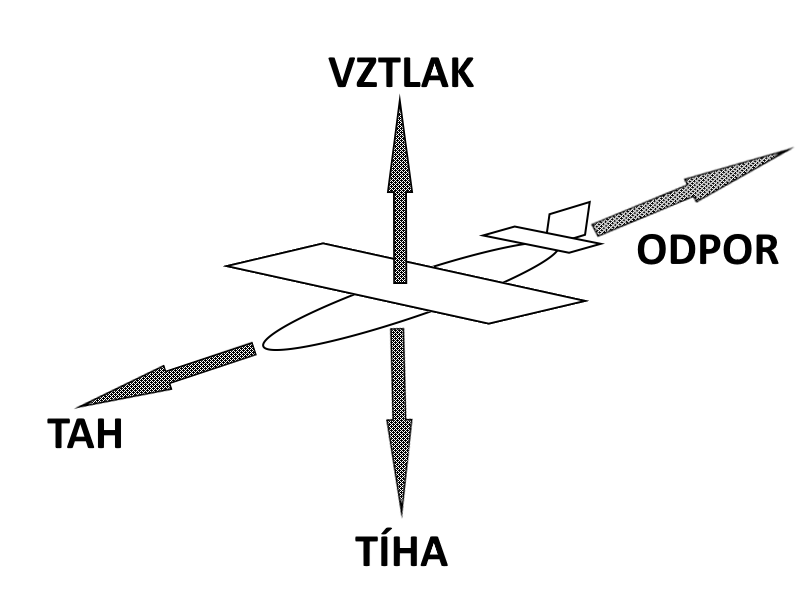
\includegraphics[width=0.55\linewidth]{sily.png}
    \caption{Čtyři základní síly působící na letadlo při letu.}
    \label{fig:sily}
\end{figure}

Tah působí ve směru letu, odpor vzduchu působí proti tahu, vztlak působí kolmo
na směr letu a~tíhová síla směřuje vždy k~zemi.

%%-------------------------------------------------------------------------
\section{Rovnováha sil v ustáleném letu}

V~ustáleném přímém letu bez zrychlení jsou síly v~rovnováze. Vztlak je roven
tíze letadla a~tah motoru vyrovnává aerodynamický odpor:

\begin{align}
    L &= W \label{eq:LW} \\
    T &= D \label{eq:TD}
\end{align}

kde $L$ je vztlak (\textit{Lift}), $W$ je tíhová síla (\textit{Weight}),
$T$ je tah (\textit{Thrust}) a~$D$ je aerodynamický odpor (\textit{Drag}).

%%-------------------------------------------------------------------------
\section{Vztlak}

\subsection{Vztlaková rovnice}

Velikost vztlaku závisí na rychlosti letu, hustotě vzduchu, ploše křídla
a~tvaru profilu. Vztlak je popsán rovnicí

\begin{equation}
    L = \frac{1}{2}\,\rho\,V^{2}\,S\,C_L
    \label{eq:lift}
\end{equation}

kde $\rho$~[\si{\kilogram\per\cubic\metre}] je hustota vzduchu,
$V$~[\si{\metre\per\second}] je rychlost letu,
$S$~[\si{\square\metre}] je plocha křídla a~$C_L$~[--] je koeficient vztlaku.

Z~rovnice~\ref{eq:lift} a~podmínky $L = W$ lze vyjádřit koeficient vztlaku
pro ustálený vodorovný let:

\begin{equation}
    C_L = \frac{2W}{\rho\,V^{2}\,S}
    \label{eq:CL}
\end{equation}

Toto je $C_L$ pro \textbf{ustálený let}. $C_{L,max}$ je pak maximální koeficient
vztlaku, při jehož překročení křídlo přestává generovat vztlak (nastává pád ---
\textit{stall}).

\subsection{Koeficient vztlaku v závislosti na úhlu náběhu}

$C_L$ roste přibližně lineárně s~úhlem náběhu $\alpha$ až do kritické hodnoty,
po jejímž překročení dochází k~odtrhnutí proudění od profilu a~prudkému
poklesu vztlaku. Tato závislost je detailně popsána v~sekci~\ref{sec:profil}.

%%-------------------------------------------------------------------------
\section{Aerodynamický odpor}

\subsection{Složky odporu}

Celkový aerodynamický odpor křídla se skládá z~profilového odporu $C_{D0}$
a~indukovaného odporu $C_{Di}$:

\begin{equation}
    C_D = C_{D0} + C_{Di}
\end{equation}

\subsection{Indukovaný odpor}

Indukovaný odpor vzniká jako důsledek tvorby vztlaku --- na koncích křídla
dochází k~přetékání vzduchu z~oblasti vysokého tlaku (pod křídlem) do oblasti
nízkého tlaku (nad křídlem), čímž vznikají koncové víry. Tyto víry způsobují
tzv. \textit{downwash} a~tím zvyšují efektivní odpor.

Indukovaný odpor je vyjádřen vztahem

\begin{equation}
    C_{Di} = \frac{C_L^2}{\pi \cdot e \cdot AR}
    \label{eq:Cdi}
\end{equation}

kde $e$~[--] je Oswaldův faktor účinnosti vyjadřující, jak blízko se reálné
rozložení vztlaku blíží ideálnímu eliptickému ($e = 1$ je ideální křídlo)
a~$AR$~[--] je štíhlost křídla (\textit{aspect ratio}):

\begin{equation}
    AR = \frac{b^2}{S}
    \label{eq:AR}
\end{equation}

kde $b$ je rozpětí křídla. Nízké $AR$ znamená vyšší indukovaný odpor,
ale lepší manévrovatelnost. Pro výpočty bylo použito $e = 0{,}85$.

%%-------------------------------------------------------------------------
\section{Profil křídla}
\label{sec:profil}

\subsection{Geometrie profilu}

Profil křídla (\textit{airfoil}) definuje tvar průřezu křídla. Základní parametry
jsou:

\begin{itemize}
    \item \textbf{Tětiva} $c$ --- vzdálenost náběžné a~odtokové hrany,
    \item \textbf{Prohnutí} (\textit{camber}) --- maximální vzdálenost střední čáry
          od tětivy, vyjadřuje se v~\% tětivy,
    \item \textbf{Tloušťka} --- maximální výška profilu v~\% tětivy,
    \item \textbf{Úhel náběhu} $\alpha$ --- úhel mezi tětivou a~vektorem rychlosti
          proudu.
\end{itemize}

\subsection{Řada NACA}

Profily řady NACA jsou systematicky pojmenovány čtyřmístným kódem NACA XYZZ,
kde:

\begin{itemize}
    \item \textbf{X} --- maximální prohnutí střednice v~\% tětivy,
    \item \textbf{Y} --- poloha maximálního prohnutí v~desetinách tětivy od náběžné hrany,
    \item \textbf{ZZ} --- maximální tloušťka profilu v~\% tětivy.
\end{itemize}

Profil s~označením NACA 0012 je tedy symetrický (nulové prohnutí),
tloušťka 12~\% tětivy. Profil NACA 4412 má prohnutí 4~\% tětivy
v~poloze 40~\% od náběžné hrany a~tloušťku 12~\%.

\subsection{Volba profilů pro tento projekt}

Pro \textbf{hlavní křídlo} byl zvolen profil \textbf{NACA 4412}. Profil má kladné prohnutí,
díky kterému generuje vztlak i~při nulovém úhlu náběhu --- to je výhodné
při nízkých rychlostech charakteristických pro tento model.

Pro \textbf{výškovku} i~\textbf{fin} byl zvolen symetrický profil \textbf{NACA 0012},
protože tyto plochy mají být aerodynamicky neutrální a~generovat sílu pouze
při výchylce z~nulové polohy.

%%-------------------------------------------------------------------------
\section{Reynoldsovo číslo}
\label{sec:reynolds}

Reynoldsovo číslo je bezrozměrný parametr popisující charakter proudění
v~mezní vrstvě:

\begin{equation}
    \Rey = \frac{V \cdot c}{\nu}
    \label{eq:Re}
\end{equation}

kde $V$~[\si{\metre\per\second}] je rychlost letu, $c$~[\si{\metre}] je tětiva
(charakteristická délka) a~$\nu$~[\si{\square\metre\per\second}] je kinematická
viskozita vzduchu ($\nu = 1{,}5 \times 10^{-5}$~\si{\square\metre\per\second}
za standardních podmínek).

Při $\Rey < 5 \times 10^5$ zůstává mezní vrstva laminární. RC modely typicky
operují v~rozsahu $\Rey \approx 10^4$--$10^5$, což přináší specifické chování:
vyšší náchylnost k~separaci laminární mezní vrstvy a~horší poměr $C_L/C_D$
ve srovnání s~velkými letadly ($\Rey > 10^6$). Tento fakt omezuje přesnost
viskózních 3D simulací v~programech jako XFLR5, proto bylo u~3D analýzy
použito inviskidní metody VLM1 a~výsledky jsou doplněny reálnými testy.

Pro návrhovou rychlost $V = 12$~\si{\metre\per\second} a~tětiva hlavního
křídla $c = 0{,}13$~\si{\metre} vychází:

\begin{equation}
    \Rey = \frac{12 \cdot 0{,}13}{1{,}5 \times 10^{-5}} \approx 104\,000
\end{equation}

Model se bude pohybovat v~rozsahu přibližně $\Rey = 80\,000$--$110\,000$.

%%-------------------------------------------------------------------------
\section{Wing loading}

Wing loading neboli zátěž na křídlo je poměr hmotnosti letadla a~plochy křídla:

\begin{equation}
    WL = \frac{m}{S}
    \label{eq:WL}
\end{equation}

kde $m$~[\si{\kilogram}] je hmotnost letadla a~$S$~[\si{\square\metre}] plocha
křídla. Nižší wing loading znamená nižší přistávací rychlost a~lepší
letové vlastnosti při nízkých rychlostech.

%%-------------------------------------------------------------------------
\section{Aerodynamická polára a klouzavost}

Aerodynamická polára zobrazuje závislost $C_L$ na $C_D$ pro různé úhly náběhu.
Klouzavost $K$ je definována jako:

\begin{equation}
    K = \frac{C_L}{C_D}
\end{equation}

Optimální pracovní bod odpovídá maximu $K$ --- letadlo letí nejúsporněji.

%%-------------------------------------------------------------------------
\section{Objemový koeficient výškovky}

Objemový koeficient výškovky (\textit{tail volume coefficient}) $V_h$ vyjadřuje
stabilizační účinek horizontálního stabilizátoru a~je klíčovým parametrem
pro nastavení podélné stability:

\begin{equation}
    V_h = \frac{S_h \cdot l_h}{S \cdot c}
    \label{eq:Vh}
\end{equation}

kde $S_h$~[\si{\square\metre}] je plocha výškovky, $l_h$~[\si{\metre}] je rameno
výškovky (vzdálenost aerodynamického středu výškovky od aerodynamického středu
hlavního křídla, počítáno u~25~\% chordu obou ploch), $S$~[\si{\square\metre}]
je plocha hlavního křídla a~$c$~[\si{\metre}] je tětiva hlavního křídla.
U~obdélníkového křídla platí $c = $ chord. Pro typická lehká letadla
se doporučuje $V_h = 0{,}3$--$0{,}7$.

%%-------------------------------------------------------------------------
\section{Objemový koeficient vertikálního stabilizátoru}

Analogicky k~$V_h$ vyjadřuje $V_v$ stabilizační účinek vertikálního
stabilizátoru (finu) ve směrové ose:

\begin{equation}
    V_v = \frac{S_v \cdot l_v}{S \cdot b}
    \label{eq:Vv}
\end{equation}

kde $S_v$~[\si{\square\metre}] je plocha finu, $l_v$~[\si{\metre}] je rameno finu,
$S$~[\si{\square\metre}] je plocha hlavního křídla a~$b$~[\si{\metre}] je rozpětí
hlavního křídla. Pro typická lehká letadla se doporučuje $V_v = 0{,}03$--$0{,}05$.

%%-------------------------------------------------------------------------
\section{Rychlost pádu}

Rychlost pádu (\textit{stall speed}) $V_{stall}$ je minimální rychlost letu,
při níž křídlo ještě generuje dostatečný vztlak. Vyplývá přímo
z~podmínky $L = W$ a~rovnice~\ref{eq:lift} pro $C_L = C_{L,max}$:

\begin{equation}
    V_{stall} = \sqrt{\frac{2\,W}{\rho\,S\,C_{L,max}}}
    \label{eq:Vstall}
\end{equation}

kde $W = mg$~[\si{\newton}] je tíhová síla letadla, $\rho = 1{,}225$~\si{\kilogram\per\cubic\metre}
je hustota vzduchu (standardní podmínky ISA) a~$C_{L,max}$~[--] je maximální koeficient
vztlaku.

Hodnotu $C_{L,max}$ pro 3D křídlo nelze přímo odečíst ze 2D simulace profilu
v~programu Xfoil, protože 2D analýza nezohledňuje koncové víry, downwash
a~nerovnoměrné rozložení vztlaku po rozpětí. Proto se 2D hodnota $C_{l,max}$
přepočítává korekčním koeficientem:

\begin{equation}
    C_{L,max} = C_{l,max} \cdot k_{3D}, \quad k_{3D} \approx 0{,}75\text{--}0{,}85
    \label{eq:CLmax3D}
\end{equation}

%%-------------------------------------------------------------------------
\section{Podélná stabilita}
\label{sec:stabilita}

\subsection{Podmínka statické stability}

Letadlo je staticky podélně stabilní, pokud těžiště (CG) leží \textbf{před}
neutrálním bodem (NP) aerodynamické konfigurace. Statická zásoba stability
(\textit{static margin}) je:

\begin{equation}
    SM = \frac{x_{NP} - x_{CG}}{\bar{c}} \cdot 100\,\%
    \label{eq:SM}
\end{equation}

kde $\bar{c}$ je střední aerodynamická tětiva. Pro RC modely se doporučuje
$SM \approx 5$--$15~\%$.

Moment koeficient $C_m$ v~závislosti na úhlu náběhu musí mít záporný sklon
$\frac{dC_m}{d\alpha} < 0$, aby letadlo samovolně vracelo nos do rovnovážné polohy.

\subsection{Řídicí plochy}

Pohyb modelu ve třech osách je řízen těmito plochami:

\begin{itemize}
    \item \textbf{Křidélka} (\textit{ailerons}) --- symetrická výchylka na obou
          křídlech v~protifázi, řídí příčné klonění (osa $x$),
    \item \textbf{Výškovka} (\textit{elevator}) --- řídí podélné kývání (osa $y$),
    \item \textbf{Směrovka} (\textit{rudder}) --- řídí stranové zatáčení (osa $z$);
          v~tomto projektu je fin pevný a~bez serva, přičemž při dané velikosti
          modelu je přímosměrná stabilita zajištěna samotnou geometrií ocasních ploch.
\end{itemize}


%%=========================================================================
%%  2. NÁVRH MODELU
%%=========================================================================
\chapter{Návrh modelu}
\label{kap:navrh}

Tato kapitola aplikuje aerodynamické vztahy z~kapitoly~1 na konkrétní geometrický
návrh modelu. Jsou zde popsány rozměry všech nosných ploch, výpočty klíčových
parametrů a~volba pohonné soustavy.

%%-------------------------------------------------------------------------
\section{Požadavky a specifikace}

Model je navržen jako RC letadlo s rozpětím křídel 600~mm a hmotností do 500~g.
Cilem je dosáhnoutí dostatečného vztlaku pro stabilní let při rychlosti 10--12~m/s, přičemž
model bude vybaven křidélky pro řízení příčného naklonění a~výškovkou pro řízení podélného kývání.
Model bude poháněn jedním bezkartáčovým motorem s~vhodnou vrtulí, přičemž poměr tahu k~hmotnosti bude vyšší než 1 pro zajištění dostatečného výkonu.

%%-------------------------------------------------------------------------
\section{Geometrie nosných ploch}

Navržené rozměry všech nosných ploch jsou shrnuty v~tabulce~\ref{tab:kridla}.

\begin{table}[H]
    \centering
    \caption{Přehled nosných ploch modelu.}
    \label{tab:kridla}
    \begin{tabular}{lrrrr}
        \toprule
        Plocha & Rozpětí & Tětiva & Profil & Plocha \\
        \midrule
        Hlavní křídlo        & 600~mm & 130~mm & NACA 4412 & $0{,}078$~m² \\
        Horizontální stabilizátor & 200~mm & 80~mm  & NACA 0012 & $0{,}016$~m² \\
        vertikální stabilizátor & 80~mm  & 80~mm  & NACA 0012 & $0{,}0064$~m² \\
        \bottomrule
    \end{tabular}
\end{table}

\subsection{Hlavní křídlo}

Hlavní křídlo má rozpětí 600~mm a~tětivu 130~mm, což dává plochu $S = 0{,}078$~m².
Použitý profil NACA~4412 zajišťuje dobré vztlakové vlastnosti a~zároveň je dostatečně
odolný vůči separaci proudění při nízkých rychlostech charakteristických pro tento model.
Štíhlost křídla dle rovnice~\ref{eq:AR} vychází $AR \approx 4{,}62$,
což je pro RC modely rozumná hodnota vyvažující indukovaný odpor a~manévrovatelnost.
Křídlo bude vybaveno křidélky (ailerony) pro řízení příčného naklonění.


\subsection{Horizontální stabilizátor}

Horizontální stabilizátor (výškovka) má rozpětí 200~mm a~tětivu 80~mm, což dává plochu $S_h = 0{,}016$~m².
Použitý profil NACA~0012 je symetrický, což je vhodné pro stabilizátor, který má být aerodynamicky neutrální.
Klapka výškovky bude výchylovatelná pro řízení náklonění nosu letadla (podélné kývání). Pro výpočet objemového 
koeficientu výškovky $V_h$ dle rovnice~\ref{eq:Vh} je třeba určit rameno $l_h$ --- vzdálenost mezi
 aerodynamickým středem hlavního křídla a~aerodynamickým středem výškovky. Při navržené geometrii a~umístění výškovky za hlavním 
 křídlem vychází $l_h \approx 0{,}29$~m, což dává $V_h \approx 0{,}45$, což je v~doporučeném rozsahu pro lehká letadla.

% ZDE --- klapky po celé délce, výpočet Vh s výsledkem 0,454

\subsection{Vertikální stabilizátor (fin)}

Vertikální stabilizátor (fin) má rozpětí 80~mm a~tětivu 80~mm, což dává plochu $S_v = 0{,}0064$~m².
Použitý profil NACA~0012 je opět symetrický, což je vhodné pro stabilizátor, který má být aerodynamicky neutrální.
Fin bude pevný, bez výchylky, protože při dané velikosti modelu a~navržené geometrii ocasních ploch je zajištěna dostatečná přímosměrná stabilita. 
Pro výpočet objemového koeficientu vertikálního stabilizátoru $V_v$ dle rovnice~\ref{eq:Vv} 
je třeba určit rameno $l_v$ --- vzdálenost mezi aerodynamickým středem hlavního křídla a~aerodynamickým středem finu vychází $l_v \approx 0{,}29$~m, což dává $V_v \approx 0{,}041$.Výsledek je v doporučeným rozsahu 
 pro lehká letadla.
% ZDE --- bez serva, pevný, výpočet Vv s výsledkem 0,041

%%-------------------------------------------------------------------------
\section{Těžiště a statická stabilita}

% ZDE --- poloha CG na 28 % MAC, postup určení, výsledek ze XFLR5,
%         Cm0 = -0,049, dCm/dalpha < 0

%%-------------------------------------------------------------------------
\section{Rychlost pádu a letové podmínky}

% ZDE --- výpočet Vstall pro clean a flaps-down,
%         návrhová rychlost 10--12 m/s, rozsah Re 80000--110000

%%-------------------------------------------------------------------------
\section{Pohonná soustava}

\subsection{Motor a vrtule}

Při výběru pohonné jednotky byly zvažovány dva motory. Prvním kandidátem byl
\textbf{MT2204}, bezkartáčový motor původně určený pro drony o~hmotnosti 25~g.
Jeho maximální tah s~vhodnou vrtulí dosahuje přibližně 440~g, nicméně vysoké
otáčky typické pro dronové motory jsou účinnější s~menšími vrtulemi (průměr
5''--6''), které jsou pro pevnokřídlé modely méně vhodné.

Jako výsledná volba byl proto zvolen motor \textbf{KAVAN Brushless C2822-1400KV},
který je přímo určen pro RC letadla. Oproti MT2204 poskytuje vyšší tah při
nižších otáčkách, je tišší a~lépe spolupracuje s~většími vrtulemi typickými
pro pevnokřídlé modely.

Výrobcem doporučená vrtule pro kombinaci s~baterií 3S je \textbf{APC 8$\times$4''}.
Tah motoru s~touto konfigurací dosahuje přibližně 500~g, z~čehož plyne poměr
tahu k~hmotnosti:

\begin{equation}
    \frac{T}{W} = \frac{500}{m_{MTOW}} \quad \text{[-]}
    \label{eq:TW}
\end{equation}

Konkrétní hodnota bude doplněna po finálním zvážení modelu. Poměr $T/W > 1$
zajišťuje dostatečný výkon pro vzlet i~vertikální stoupání.

\subsection{Regulátor ESC a baterie}

Pro regulaci otáček motoru je použit elektronický regulátor \textbf{Hornet 40A}
(2--4S), který komunikuje s~řídící jednotkou pomocí standardního PWM signálu.
Napájení zajišťuje baterie \textbf{KAVAN LiPo 1300~mAh / 11{,}1~V (3S) / 40--80C}.
Jmenovité napětí 11{,}1~V a~kapacita 1300~mAh představují dobrý kompromis
mezi hmotností a~výdrží.

\subsection{Energetická bilance}

% ZDE --- odhadovaná doba letu

%%-------------------------------------------------------------------------
\section{Konstrukce a použité materiály}

\subsection{Drak křídla}

Při návrhu konstrukčního řešení křídla byly zvažovány dvě možnosti.

\textbf{Možnost A --- žebra s~uhlíkovými nosníky a~fólií.}
Žebra odpovídající profilu NACA 4412 jsou tištěna na FDM tiskárně
s~odlehčovacími otvory. Skrze žebra procházejí dva uhlíkové nosníky
(průměr 6~mm, délka 600~mm), které zajišťují torzní i~ohybovou tuhost křídla.
Povrch je potažen smršťovací fólií, která vytváří aerodynamicky hladký povrch
a~přidává minimální hmotnost. Výsledná konstrukce je pevná, tvarově konzistentní
a~lehká.

\textbf{Možnost B --- tisk celého křídla z~LW-PLA.}
Speciální materiál LW-PLA (Light Weight PLA) při tisku expanduje a~vytváří
pěnovou strukturu s~výrazně nižší hustotou než standardní PLA. Tisk křídla
jako celku by poskytl dokonalý tvar profilu bez nutnosti potahování. Hlavní
nevýhodou je požadavek na nepřerušovaný tisk --- jakékoli přerušení způsobí
viditelnou vadu na povrchu. Skrze trup by i~v~tomto případě procházela uhlíková
tyč jako hlavní nosný prvek.

Pro tento projekt byla zvolena \textbf{možnost A} jako konstrukčně spolehlivější
a~snadněji opravitelná.

\subsection{Trup}

Hlavní část trupu tvoří čtvercový profil z~uhlíkového kompozitu s~tloušťkou stěn 1~mm
a~rozměry $20 \times 20 \times 355$~mm. Tato konstrukce poskytuje vysokou tuhost
při minimální hmotnosti. Na obou stranách tyče jsou přilepeny dřevěné příložky,
které slouží jako montážní body pro hlavní křídlo a~jako nosič elektroniky.
Na druhém konci tyče je zasunut horizontální stabilizátor, připevněný pomocí šroubů.
Vertikální stabilizátor (fin) je přilepen k~horizontálnímu stabilizátoru
a~zůstává pevný bez serva.

\subsection{Ocasní plochy}

Ocasní plochy jsou vytištěny na 3D tiskárně z~PLA s~nízkým procentem výplně,
přičemž přesný tvar profilu NACA~0012 je zachován po celé délce. Výškovka
(\textit{elevator}) je ovládána servomotorem MG90S, zatímco fin zůstává pevný
bez serva. Přímosměrná stabilita je zajištěna samotnou geometrií ocasních ploch,
což zjednodušuje konstrukci a~snižuje celkovou hmotnost modelu.

\subsection{Uchycení křídla k trupu}

Uhlíkové tyče procházejí žebry křídla a~jsou pevně přilepeny epoxidovým lepidlem.
Křídlo je k~trupu připevněno pomocí dvou dřevěných příložek, které jsou šrouby
uchyceny k~uhlíkové tyči trupu. Ocasní plochy jsou vytištěny jako celky
a~připevněny k~trupu kombinací šroubů a~lepidla.
\subsection{Výrobní postup}

% ZDE --- postup krok za krokem + fotodokumentace


%%=========================================================================
%%  3. ELEKTRONIKA
%%=========================================================================
\chapter{Elektronika}

Palubní elektronika modelu tvoří dva samostatné celky --- \textbf{letadlo}
a~\textbf{ovladač} --- propojené bezdrátovou komunikací přes moduly HC-12.
Tato kapitola popisuje všechny použité součástky, schéma zapojení
a~napájecí architekturu obou celků. Podrobný popis softwarové části
je uveden v~kapitole~4.

%%-------------------------------------------------------------------------
\section{Blokové schéma systému}

% ZDE --- vložit obrázek blokového schématu

%%-------------------------------------------------------------------------
\section{Přehled součástek}

Tabulky~\ref{tab:parts_letadlo} a~\ref{tab:parts_ovladac} shrnují
všechny klíčové součástky obou celků.

\begin{table}[H]
    \centering
    \caption{Součástky --- letadlo.}
    \label{tab:parts_letadlo}
    \begin{tabular}{ll}
        \toprule
        Součástka & Popis \\
        \midrule
        ESP32 (WROOM)         & Hlavní řídící jednotka \\
        HC-12 (433~MHz)       & Bezdrátový přijímač \\
        MG90S $\times$ 3      & Servomotory (křídla, výškovka) \\
        Hornet 40A ESC        & Regulátor otáček motoru \\
        KAVAN C2822-1400KV    & Bezkartáčový motor \\
        LiPo 3S 1300~mAh      & Hlavní baterie \\
        Kondenzátor $\sim$700~\si{\micro\farad} & Filtrace rušení u~ESP32 \\
        \bottomrule
    \end{tabular}
\end{table}

\begin{table}[H]
    \centering
    \caption{Součástky --- ovladač.}
    \label{tab:parts_ovladac}
    \begin{tabular}{ll}
        \toprule
        Součástka & Popis \\
        \midrule
        ESP32                         & Řídící jednotka ovladače \\
        HC-12 (433~MHz)               & Bezdrátový vysílač \\
        Joystick 1              & Řízení zatáčení (roll/yaw) \\
        Joystick 2 & Řízení plynu (throttle) \\
        Powerbanka                    & Napájení ovladače \\
        \bottomrule
    \end{tabular}
\end{table}

%%-------------------------------------------------------------------------
\section{Popis součástek}
 
\subsection{Mikrokontrolér ESP32}
 
ESP32 je 32bitový mikrokontrolér od společnosti Espressif Systems
s~dvoujádrovým procesorem Xtensa LX6 taktovaným na 240~MHz.
Pro tento projekt je klíčová dostupnost více hardwarových rozhraní
UART a 12bitový ADC pro čtení analogových vstupů
a~dostatečný počet PWM výstupů pro řízení serv a~ESC.
Mikrokontrolér je použit jak v~letadle (přijímač), tak v~ovladači (vysílač),
což zjednodušuje vývoj firmware --- obě zařízení sdílejí stejnou platformu
a~vývojové prostředí Arduino IDE.
 
\subsection{Bezdrátový modul HC-12}
 
HC-12 je hotový bezdrátový transceiver pracující v~pásmu 433~MHz,
podrobně popsaný v~sekci~4.2. Z~pohledu hardwarového zapojení
se jedná o~5pinový modul (VCC, GND, TXD, RXD, SET) komunikující
přes rozhraní UART s~napájecím napětím 3{,}2--5{,}5~V.
Modul obsahuje integrovanou anténu, kterou lze v~případě potřeby
nahradit externí pro zvýšení dosahu. Pro tento projekt je však integrovaná anténa zcela dostačující.
 
\subsection{Servomotory MG90S}
 
MG90S je miniaturní servomotor s~kovovými převody o~hmotnosti 13{,}4~g.
Oproti plastovým převodům poskytuje vyšší odolnost vůči rázu při přistání
a~delší životnost při opakovaném zatížení. Základní parametry jsou
shrnuty v~tabulce~\ref{tab:mg90s}.
 
\begin{table}[H]
    \centering
    \caption{Parametry servomotoru MG90S.}
    \label{tab:mg90s}
    \begin{tabular}{ll}
        \toprule
        Parametr & Hodnota \\
        \midrule
        Napájecí napětí   & 4{,}8--6{,}0~V \\
        Krouticí moment   & 1{,}8~kg$\cdot$cm (při 4{,}8~V) \\
        Rychlost          & 0{,}1~s / 60° (při 4{,}8~V) \\
        Hmotnost          & 13{,}4~g \\
        Rozhraní          & PWM 50~Hz, pulz 1000--2000~\si{\micro\second} \\
        \bottomrule
    \end{tabular}
\end{table}
 
V~modelu jsou použity celkem tři kusy MG90S: dva pro křidélka
a~jeden pro výškovku.

\subsection{Joystiky}

Ovladač je vybaven dvěma dvouosými joystiky, 
ketré fungují na principu potenciometrů. Jeden joystick řídí zatáčení (roll/yaw) a~druhý řídí plyn (throttle). 
Výstupy z~joysticků jsou čteny jako analogové hodnoty pomocí ADC pinů na ESP32, které jsou následně mapovány na odpovídající rozsah PWM signálu a~odesílány přes HC-12 do letadla.
 
\subsection{Regulátor ESC a motor}
 
Elektronický regulátor otáček \textbf{Hornet 40A} (2--4S LiPo) řídí
bezkartáčový motor pomocí třífázového PWM signálu. Vstupní signál
z~ESP32 je standardní servo PWM (50~Hz, 1000--2000~\si{\micro\second}),
kde 1000~\si{\micro\second} odpovídá nulovým otáčkám a~2000~\si{\micro\second}
plnému plynu. ESC obsahuje integrovaný BEC (\textit{Battery Eliminator Circuit}),
který bude sloužit jako zdroj 5~V pro ESP32 a ostatní elektroniku.
 
Motor \textbf{KAVAN Brushless C2822-1400KV} je bezkartáčový motor
s~hodnotou KV udávající počet otáček za minutu na volt napájecího napětí.
Při napájení z~3S LiPo (11{,}1~V) jsou tak teoretické volnoběžné otáčky
přibližně $1400 \times 11{,}1 \approx 15\,500$~ot/min.
Maximální tah s~vrtulí APC 8$\times$4'' na 3S dosahuje přibližně 500~g.
 
\subsection{Napájení --- LiPo baterie}
 
Hlavním zdrojem energie je baterie \textbf{KAVAN LiPo 1300~mAh / 11{,}1~V (3S) / 40--80C}.
Trojčlánková konfigurace (3S) poskytuje jmenovité napětí 11{,}1~V
a~plně nabitý stav 12{,}6~V. Vybíjecí schopnost 40C znamená,
že baterie dokáže trvale dodávat proud až 52~A,
což s~rezervou pokryje potřeby motoru i~elektroniky. 

%%-------------------------------------------------------------------------
\section{Schéma zapojení}

% ZDE --- odkaz na přílohu nebo vložit přímo

%%=========================================================================
%%  4. SOFTWARE A KOMUNIKACE
%%=========================================================================
\chapter{Software a komunikace}

Tato kapitola popisuje softwarovou architekturu systému dálkového ovládání.
Komunikace mezi ovladačem a~letadlem je realizována přes moduly HC-12
pracující na frekvenci 433~MHz. Kapitola dále obsahuje strukturu
a~klíčové části firmware obou zařízení.

%%-------------------------------------------------------------------------
\section{Architektura systému}

Systém se skládá ze dvou nezávislých zařízení. \textbf{Ovladač} čte hodnoty
z~páček a~joysticků, zabalí je do datové struktury a~odesílá bezdrátově
přes HC-12. \textbf{Přijímač} v~letadle čeká na příchozí pakety, dekóduje je
a~nastaví odpovídající polohy serv a~otáčky motoru. Oba uzly používají
mikrokontrolér ESP32 a~identické moduly HC-12.

%%-------------------------------------------------------------------------
\section{Komunikační modul HC-12}

\subsection{Princip funkce a parametry}

HC-12 je hotový bezdrátový modul pracující v~pásmu \textbf{433~MHz}
s~integrovaným rádiovým čipem Si4463. Z~pohledu mikrokontroléru se chová
jako standardní sériová linka (UART) --- co přijde na pin TX, objeví se na
pinu RX druhého modulu. Není tedy potřeba řešit žádné RF parametry ani
instalovat speciální knihovny. Dosah modulu v~přímé viditelnosti dosahuje
stovky metrů, což pro účely tohoto projektu plně dostačuje.

Klíčové parametry modulu jsou shrnuty v~tabulce~\ref{tab:hc12}.

\begin{table}[H]
    \centering
    \caption{Parametry modulu HC-12.}
    \label{tab:hc12}
    \begin{tabular}{ll}
        \toprule
        Parametr & Hodnota \\
        \midrule
        Frekvenční pásmo    & 433{,}4--473{,}0~MHz \\
        Napájecí napětí     & 3{,}2--5{,}5~V \\
        Výchozí baudrate    & 9600~Bd \\
        Výkon vysílače      & až 20~dBm (100~mW) \\
        Rozhraní            & UART (TTL) \\
        \bottomrule
    \end{tabular}
\end{table}

\subsection{Konfigurace modulu}

HC-12 se konfiguruje pomocí AT příkazů při přivedení pinu SET do logické
nuly. V~běžném provozu je SET v~logické jedničce a~modul transparentně
přeposílá data. Pro tento projekt je použito výchozí nastavení
(9600~Bd, kanál 1), které nevyžaduje žádnou změnu konfigurace.

Zapojení HC-12 k~ESP32 je na obou stranách (ovladač i~letadlo) identické:

\begin{itemize}
    \item \textbf{VCC} $\rightarrow$ 3{,}3~V
    \item \textbf{GND} $\rightarrow$ GND
    \item \textbf{TXD} (HC-12) $\rightarrow$ RX (ESP32)
    \item \textbf{RXD} (HC-12) $\rightarrow$ TX (ESP32)
    \item \textbf{SET} $\rightarrow$ HIGH (běžný provoz)
    \item \textbf{ANT} $\rightarrow$ anténa
\end{itemize}

\subsection{Formát přenášených dat}

Řídicí hodnoty jsou přenášeny jako binární datová struktura
(\textit{struct}). Binární přenos je efektivnější než textový formát
(např. CSV) --- přenáší se přesně 8~bajtů místo desítek ASCII znaků,
čímž se snižuje latence.

\begin{lstlisting}[style=c_style, caption={Datová struktura řídicího paketu.}]
struct Data {
    int16_t throttle;  // plyn:     0 az 1000
    int16_t pitch;     // vyskovka: -500 az +500
    int16_t roll;      // kridela:  -500 az +500
    int16_t yaw;       // smerovka: -500 az +500
};
\end{lstlisting}

Použití typu \texttt{int16\_t}, což je 16bitové celé číslo se znaménkem,
zajišťuje přesnost kroků a~konstantní velikost 2~bajty
na kanál nezávisle na platformě.

%%-------------------------------------------------------------------------
\section{Kód vysílače (ovladač)}

\subsection{Struktura kódu}

Software ovladače provádí v~hlavní smyčce tři operace: přečte aktuální
hodnoty z~analogových vstupů, uloží je do struktury \texttt{Data}
a~odešle strukturu jako blok bajtů přes HC-12. Smyčka se opakuje
přibližně každých 50~ms, čímž je dosaženo odesílací frekvence 20~Hz.

\subsection{Čtení vstupů}

Joystick 1 poskytuje dva analogové výstupy (osy X a~Y) v~rozsahu
0--3{,}3~V. Joystick 2 slouží jako ovladač plynu. Hodnoty jsou
čteny přes 12bitový ADC ESP32 a~mapovány na rozsah odpovídající
datové struktuře.

\subsection{Odesílání dat}

\begin{lstlisting}[style=c_style, caption={Odesílání paketu z ovladače.}]

\end{lstlisting}

%%-------------------------------------------------------------------------
\section{Kód přijímače (letadlo)}

\subsection{Příjem a dekódování dat}

Přijímač čeká, dokud není v~bufferu k~dispozici celý paket (8~bajtů).
Jakmile data dorazí, přečte je do struktury \texttt{ControlPacket}
a~předá dál k~řízení serv a~ESC.

\begin{lstlisting}[style=c_style, caption={Příjem paketu na straně letadla.}]

\end{lstlisting}

\subsection{Řízení servomotorů a ESC}

Servomotory i~ESC jsou řízeny PWM signálem s~periodou 20~ms
(frekvence 50~Hz). Šířka pulzu v~rozsahu 1000--2000~\si{\micro\second}
odpovídá plnému rozsahu pohybu serva nebo plynu motoru.
Hodnoty z~přijatého paketu jsou mapovány na tento rozsah
a~předány příslušným výstupním pinům ESP32.

\subsection{Fail-safe}

Do budoucna je plánováno přidání \textbf{fail-safe módu}: pokud nepřijde
žádný paket po dobu delší než stanovený timeout, firmware automaticky
nastaví nulový plyn a~vycentruje všechna serva. Tím se zamezí nekontrolovanému
letu v~případě výpadku spojení.

%%-------------------------------------------------------------------------
\section{Ovladač --- hardwarová realizace}

% ZDE --- popis fyzické podoby ovladače, rozmístění komponent


%%=========================================================================
%%  ZÁVĚR
%%=========================================================================
\clearpage
\chapter*{Závěr}
\addcontentsline{toc}{chapter}{Závěr}

% ZDE


%%=========================================================================
%%  LITERATURA
%%=========================================================================
\begin{thebibliography}{99}
\addcontentsline{toc}{chapter}{Literatura}

% \bibitem{klic} PŘÍJMENÍ, Jméno. \emph{Název}. Místo: Nakladatel, rok. ISBN ...

\end{thebibliography}


%%=========================================================================
%%  PŘÍLOHY
%%=========================================================================
\chapter*{Přílohy}
\pagenumbering{Roman}
\addcontentsline{toc}{chapter}{Přílohy}

\section*{Příloha I --- Schéma zapojení}
% ZDE

\section*{Příloha II --- Zdrojový kód}
% ZDE nebo odkaz na GitLab

\section*{Příloha III --- Fotodokumentace}
% ZDE

\end{document}